\documentclass[
  man,
  floatsintext,
  longtable,
  nolmodern,
  notxfonts,
  notimes,
  colorlinks=true,linkcolor=blue,citecolor=blue,urlcolor=blue]{apa7}

\usepackage{amsmath}
\usepackage{amssymb}



\usepackage[bidi=default]{babel}
\babelprovide[main,import]{american}


% get rid of language-specific shorthands (see #6817):
\let\LanguageShortHands\languageshorthands
\def\languageshorthands#1{}

\RequirePackage{longtable}
\RequirePackage{threeparttablex}

\makeatletter
\renewcommand{\paragraph}{\@startsection{paragraph}{4}{\parindent}%
	{0\baselineskip \@plus 0.2ex \@minus 0.2ex}%
	{-.5em}%
	{\normalfont\normalsize\bfseries\typesectitle}}

\renewcommand{\subparagraph}[1]{\@startsection{subparagraph}{5}{0.5em}%
	{0\baselineskip \@plus 0.2ex \@minus 0.2ex}%
	{-\z@\relax}%
	{\normalfont\normalsize\bfseries\itshape\hspace{\parindent}{#1}\textit{\addperi}}{\relax}}
\makeatother




\usepackage{longtable, booktabs, multirow, multicol, colortbl, hhline, caption, array, float, xpatch}
\usepackage{subcaption}


\renewcommand\thesubfigure{\Alph{subfigure}}
\setcounter{topnumber}{2}
\setcounter{bottomnumber}{2}
\setcounter{totalnumber}{4}
\renewcommand{\topfraction}{0.85}
\renewcommand{\bottomfraction}{0.85}
\renewcommand{\textfraction}{0.15}
\renewcommand{\floatpagefraction}{0.7}

\usepackage{tcolorbox}
\tcbuselibrary{listings,theorems, breakable, skins}
\usepackage{fontawesome5}

\definecolor{quarto-callout-color}{HTML}{909090}
\definecolor{quarto-callout-note-color}{HTML}{0758E5}
\definecolor{quarto-callout-important-color}{HTML}{CC1914}
\definecolor{quarto-callout-warning-color}{HTML}{EB9113}
\definecolor{quarto-callout-tip-color}{HTML}{00A047}
\definecolor{quarto-callout-caution-color}{HTML}{FC5300}
\definecolor{quarto-callout-color-frame}{HTML}{ACACAC}
\definecolor{quarto-callout-note-color-frame}{HTML}{4582EC}
\definecolor{quarto-callout-important-color-frame}{HTML}{D9534F}
\definecolor{quarto-callout-warning-color-frame}{HTML}{F0AD4E}
\definecolor{quarto-callout-tip-color-frame}{HTML}{02B875}
\definecolor{quarto-callout-caution-color-frame}{HTML}{FD7E14}

%\newlength\Oldarrayrulewidth
%\newlength\Oldtabcolsep


\usepackage{hyperref}




\providecommand{\tightlist}{%
  \setlength{\itemsep}{0pt}\setlength{\parskip}{0pt}}
\usepackage{longtable,booktabs,array}
\usepackage{calc} % for calculating minipage widths
% Correct order of tables after \paragraph or \subparagraph
\usepackage{etoolbox}
\makeatletter
\patchcmd\longtable{\par}{\if@noskipsec\mbox{}\fi\par}{}{}
\makeatother
% Allow footnotes in longtable head/foot
\IfFileExists{footnotehyper.sty}{\usepackage{footnotehyper}}{\usepackage{footnote}}
\makesavenoteenv{longtable}

\usepackage{graphicx}
\makeatletter
\newsavebox\pandoc@box
\newcommand*\pandocbounded[1]{% scales image to fit in text height/width
  \sbox\pandoc@box{#1}%
  \Gscale@div\@tempa{\textheight}{\dimexpr\ht\pandoc@box+\dp\pandoc@box\relax}%
  \Gscale@div\@tempb{\linewidth}{\wd\pandoc@box}%
  \ifdim\@tempb\p@<\@tempa\p@\let\@tempa\@tempb\fi% select the smaller of both
  \ifdim\@tempa\p@<\p@\scalebox{\@tempa}{\usebox\pandoc@box}%
  \else\usebox{\pandoc@box}%
  \fi%
}
% Set default figure placement to htbp
\def\fps@figure{htbp}
\makeatother


% definitions for citeproc citations
\NewDocumentCommand\citeproctext{}{}
\NewDocumentCommand\citeproc{mm}{%
  \begingroup\def\citeproctext{#2}\cite{#1}\endgroup}
\makeatletter
 % allow citations to break across lines
 \let\@cite@ofmt\@firstofone
 % avoid brackets around text for \cite:
 \def\@biblabel#1{}
 \def\@cite#1#2{{#1\if@tempswa , #2\fi}}
\makeatother
\newlength{\cslhangindent}
\setlength{\cslhangindent}{1.5em}
\newlength{\csllabelwidth}
\setlength{\csllabelwidth}{3em}
\newenvironment{CSLReferences}[2] % #1 hanging-indent, #2 entry-spacing
 {\begin{list}{}{%
  \setlength{\itemindent}{0pt}
  \setlength{\leftmargin}{0pt}
  \setlength{\parsep}{0pt}
  % turn on hanging indent if param 1 is 1
  \ifodd #1
   \setlength{\leftmargin}{\cslhangindent}
   \setlength{\itemindent}{-1\cslhangindent}
  \fi
  % set entry spacing
  \setlength{\itemsep}{#2\baselineskip}}}
 {\end{list}}
\usepackage{calc}
\newcommand{\CSLBlock}[1]{\hfill\break\parbox[t]{\linewidth}{\strut\ignorespaces#1\strut}}
\newcommand{\CSLLeftMargin}[1]{\parbox[t]{\csllabelwidth}{\strut#1\strut}}
\newcommand{\CSLRightInline}[1]{\parbox[t]{\linewidth - \csllabelwidth}{\strut#1\strut}}
\newcommand{\CSLIndent}[1]{\hspace{\cslhangindent}#1}





\usepackage{newtx}

\defaultfontfeatures{Scale=MatchLowercase}
\defaultfontfeatures[\rmfamily]{Ligatures=TeX,Scale=1}





\title{Small Errors, Big Consequences: Lessons from Data Mismanagement
in Business}


\shorttitle{Small Errors, Big Consequences}


\usepackage{etoolbox}






\author{Alireza Toutounchi (Matriculation:400889526)}



\affiliation{
{Hochschule Fresenius - University of Applied Science}}




\leftheader{(Matriculation:400889526)}



\abstract{In the era of data-driven decision-making, even minor errors
in data management can lead to major financial, operational, and
reputational consequences for businesses. This paper explores real-world
cases where inaccurate, incomplete, or poorly governed data resulted in
substantial setbacks for global organizations. Through an analysis of
incidents at companies such as Equifax, Unity Technologies, Samsung, and
Knight Capital, we highlight how flawed data inputs, system failures,
and human errors have led to multimillion-dollar losses, regulatory
penalties, and public mistrust. The study also presents a simulation
comparing true and faulty forecasts in business reporting to illustrate
how data errors can distort insights and decisions. Finally, key lessons
are drawn, emphasizing the critical importance of robust data
governance, validation systems, and proactive error detection in
maintaining business integrity and resilience. }

\keywords{Data, Errors, Consequences, Mismanagement, Analysis}

\authornote{ 
\par{ }
\par{   The authors have no conflicts of interest to disclose.    }
\par{Correspondence concerning this article should be addressed
to Alireza Toutounchi
(Matriculation:400889526), Email: \href{mailto:toutounchi.alireza@stud.hs-fresenius.de}{toutounchi.alireza@stud.hs-fresenius.de}}
}

\makeatletter
\let\endoldlt\endlongtable
\def\endlongtable{
\hline
\endoldlt
}
\makeatother

\urlstyle{same}



\makeatletter
\@ifpackageloaded{caption}{}{\usepackage{caption}}
\AtBeginDocument{%
\ifdefined\contentsname
  \renewcommand*\contentsname{Table of contents}
\else
  \newcommand\contentsname{Table of contents}
\fi
\ifdefined\listfigurename
  \renewcommand*\listfigurename{List of Figures}
\else
  \newcommand\listfigurename{List of Figures}
\fi
\ifdefined\listtablename
  \renewcommand*\listtablename{List of Tables}
\else
  \newcommand\listtablename{List of Tables}
\fi
\ifdefined\figurename
  \renewcommand*\figurename{Figure}
\else
  \newcommand\figurename{Figure}
\fi
\ifdefined\tablename
  \renewcommand*\tablename{Table}
\else
  \newcommand\tablename{Table}
\fi
}
\@ifpackageloaded{float}{}{\usepackage{float}}
\floatstyle{ruled}
\@ifundefined{c@chapter}{\newfloat{codelisting}{h}{lop}}{\newfloat{codelisting}{h}{lop}[chapter]}
\floatname{codelisting}{Listing}
\newcommand*\listoflistings{\listof{codelisting}{List of Listings}}
\makeatother
\makeatletter
\makeatother
\makeatletter
\@ifpackageloaded{caption}{}{\usepackage{caption}}
\@ifpackageloaded{subcaption}{}{\usepackage{subcaption}}
\makeatother

% From https://tex.stackexchange.com/a/645996/211326
%%% apa7 doesn't want to add appendix section titles in the toc
%%% let's make it do it
\makeatletter
\xpatchcmd{\appendix}
  {\par}
  {\addcontentsline{toc}{section}{\@currentlabelname}\par}
  {}{}
\makeatother

%% Disable longtable counter
%% https://tex.stackexchange.com/a/248395/211326

\usepackage{etoolbox}

\makeatletter
\patchcmd{\LT@caption}
  {\bgroup}
  {\bgroup\global\LTpatch@captiontrue}
  {}{}
\patchcmd{\longtable}
  {\par}
  {\par\global\LTpatch@captionfalse}
  {}{}
\apptocmd{\endlongtable}
  {\ifLTpatch@caption\else\addtocounter{table}{-1}\fi}
  {}{}
\newif\ifLTpatch@caption
\makeatother

\begin{document}

\maketitle

\hypertarget{toc}{}
\tableofcontents
\newpage
\section[Introduction]{Small Errors, Big Consequences: Lessons from Data
Mismanagement in Business}

\setcounter{secnumdepth}{-\maxdimen} % remove section numbering

\setlength\LTleft{0pt}


The term ``data'' refers to raw facts, figures, or information collected
for reference, analysis, or processing. Data can exist in many forms ---
numbers, text, images, audio, video, or symbols --- and it has no
meaning on its own until it is interpreted.

\textbf{Types of Data:}

\begin{enumerate}
\def\labelenumi{\arabic{enumi}.}
\tightlist
\item
  Quantitative Data (Numerical)
\end{enumerate}

● Discrete: Countable (e.g., number of students).

● Continuous: Measurable (e.g., height, weight).

\begin{enumerate}
\def\labelenumi{\arabic{enumi}.}
\setcounter{enumi}{1}
\tightlist
\item
  Qualitative Data (Categorical)
\end{enumerate}

●Nominal: Categories with no order (e.g., gender, color).

●Ordinal: Categories with order (e.g., satisfaction level: low, medium,
high).

\textbf{Forms of Data:} • Structured (organized in tables like Excel or
databases) • Unstructured (like emails, social media, videos) •
Semi-structured (like JSON or XML files)

(\citeproc{ref-provost2013data}{Provost \& Fawcett, 2013})

\begin{longtable}[]{@{}rlll@{}}
\toprule\noalign{}
ID & Name & Department & Salary \\
\midrule\noalign{}
\endhead
\bottomrule\noalign{}
\endlastfoot
102 & Jane & HR & €3,500 \\
\end{longtable}

This becomes information when we interpret it --- for example,
understanding that Jane works in HR and earns €3,500. The most basic
division of information is good and bad information. This distinction is
crucial in fields like data science, business intelligence,
decision-making, and information systems.

\subsection{Good Information}\label{good-information}

Good information is accurate, timely, relevant, complete, and reliable.
It enhances decision-making and contributes to achieving goals.

\begin{enumerate}
\def\labelenumi{\arabic{enumi}.}
\tightlist
\item
  Accuracy -- Free from error.
\item
  Timeliness -- Up to date and delivered on time.
\item
  Relevance -- Applicable to the problem or decision at hand.
\item
  Completeness -- Covers all important facts.
\item
  Reliability -- Trustworthy and consistent.
\end{enumerate}

Example: A dashboard showing real-time sales performance across regions
using verified data sources.

\subsection{Bad Information}\label{bad-information}

Bad information is inaccurate, outdated, irrelevant, incomplete, or
misleading. It leads to poor decisions and potentially serious
consequences. 1. Misinformation -- False or misleading information
shared without harmful intent. 2. Disinformation -- Deliberately
deceptive information shared with malicious intent. 3. Outdated data --
Information that was once correct but no longer reflects the current
state.

Example: Using last year's market trends to make decisions in a rapidly
changing economy without checking current data.

\textbf{The topic of discussion here is bad information, so I will
address this issue and examine its implications and delve into it a
little deeper.}

Bad data can cost you money. It can also damage your reputation, drive
good customers away, and negatively affect your entire workforce. Bad
data, more often than not, results in bad decisions -- and bad decisions
can destroy a business. The true costs of bad data are so overwhelming
that they are scary. If you do not take data quality seriously, you are
at risk of being blindsided by the enormous impact of bad data.

\textbf{What is Bad Data?}

Bad data is any data that is not wholly accurate or doesn't conform to
necessary standards. That can include inaccurate data, incomplete data,
conflicting data, duplicate data, invalid data, and unsynchronized data.

(\citeproc{ref-firsteigen_cost_bad_data}{\textbf{firsteigen\_cost\_bad\_data?}})

\textbf{Example of bad data}

\begin{verbatim}

Attaching package: 'dplyr'
\end{verbatim}

\begin{verbatim}
The following objects are masked from 'package:stats':

    filter, lag
\end{verbatim}

\begin{verbatim}
The following objects are masked from 'package:base':

    intersect, setdiff, setequal, union
\end{verbatim}

\begin{verbatim}
Warning: Using `size` aesthetic for lines was deprecated in ggplot2 3.4.0.
i Please use `linewidth` instead.
\end{verbatim}

\pandocbounded{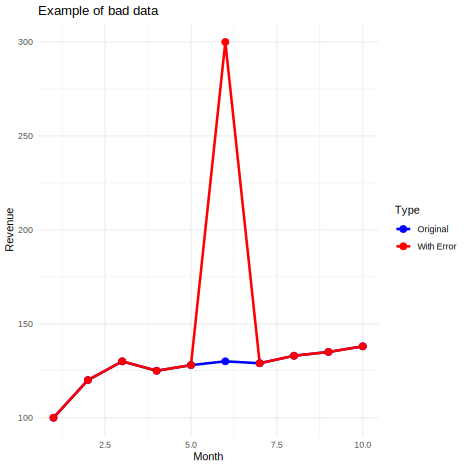
\includegraphics[keepaspectratio]{small-errors-big-consequences-final_files/figure-pdf/unnamed-chunk-2-1.pdf}}

\textbf{How bad data can impact your businesses ?}

This is the most important question you should be concerned with to
reach the correct answer in terms of proper management and preventing
significant damage from the smallest errors. To answer this question, I
would say that if the initial errors are recoverable with a small error
margin and the project is flexible, it may be possible to prevent the
issue with minimal cost and in the shortest possible time. However, if
we analyze it on paper, if a project that is already in progress has not
been properly analyzed beforehand and its roadmap hasn't been prepared,
even if the error is addressed quickly, the project will still face
significant consequences.

(\citeproc{ref-firsteigen_cost_bad_data}{\textbf{firsteigen\_cost\_bad\_data?}})

\begin{figure}[H]

\caption{Fig2.Table1}

{\centering \pandocbounded{\includegraphics[keepaspectratio]{002.png}}

}

\end{figure}%

\textbf{How does your business use data?}

It outlines two primary functions of business data use---Making
decisions and Managing operations---and illustrates the negative
consequences of poor data practices under each.

\textbf{1. Making Decisions}

Businesses rely heavily on data to guide strategic, operational, and
financial decisions. When data is incomplete, outdated, or incorrect, it
leads to:

\textbf{• Poor decisions:} Executives may act on flawed insights,
leading to failed investments or ineffective campaigns.

\textbf{• Missed opportunities:} Without timely or accurate data,
organizations may overlook market trends or emerging customer needs.

\textbf{• Internal loss of trust:} Employees lose confidence in systems
or leadership when data repeatedly proves unreliable.

Example:

A retail company might misinterpret sales data due to duplicate entries,
leading to overproduction of a poorly performing product.

\textbf{2. Managing Operations}

Data also plays a key role in the day-to-day functioning of a
business---like inventory control, customer support, and supply chain
management.

When data is mismanaged, it results in:

\textbf{• Wasted time \& money:} Teams spend hours cleaning, verifying,
or reconciling data.

\textbf{• Frustrated customers:} Inaccurate customer profiles or slow
systems erode user experience.

\textbf{• External loss of trust:} Repeated failures caused by bad data
can harm a brand's reputation in the market.

Example:

An e-commerce platform using outdated shipping data may send packages to
the wrong addresses, frustrating customers and increasing return costs.

\textbf{Conclusion:}

Businesses depend on data to inform both decision-making and daily
operations. when this data is unreliable, the consequences ripple
through every layer of the organization---from strategic planning to
customer satisfaction. Mismanagement not only wastes resources but
undermines trust both internally and externally. Companies must treat
data as a critical asset, investing in quality controls, validation
systems, and data governance to mitigate these risks.

\textbf{What is Data Normalizing ?}

Data normalization is the process of scaling numerical values so that
they fall within a common range---often between 0 and 1 or so they have
a mean of 0 and a standard deviation of 1.

(\citeproc{ref-smith2025impactdata}{\textbf{smith2025impactdata?}})

\textbf{When use ?}

When we want to perform the process of scaling numerical values for
numerical data (numeric variables), we can use data normalization.
However, for some data that are not numerical, such as categorical data
(gender and country), we simply need to encode the data, and binary data
(0, 1) are usually already normalized. Textual and historical data must
first be converted into numerical features.

The following algorithms are commonly used for normalization:

• K-means clustering

• PCA

• Logistic / Linear Regression

• SVM

• Neural Networks

• Decision Tree / Random Forest

(\citeproc{ref-provost2013researchgate}{\textbf{provost2013researchgate?}})

\begin{verbatim}
# A tibble: 6 x 5
  Sales Employees Expenses Profit Customer_Satisfaction
  <int>     <int>    <int>  <int>                 <dbl>
1  3608         7     1815   1126                  9.4 
2  3368        45     1335    473                  9.33
3  2176        93     1481    869                  7.61
4  2097        31     2693   1114                  4   
5  2251        40     1871    797                  5.64
6  4217        99     2744    749                  7.7 
\end{verbatim}

\pandocbounded{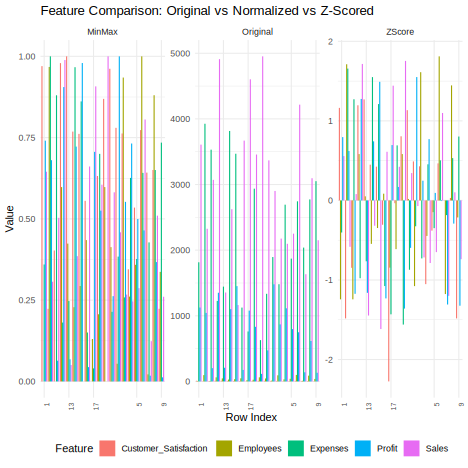
\includegraphics[keepaspectratio]{small-errors-big-consequences-final_files/figure-pdf/unnamed-chunk-4-1.pdf}}

The table above includes:

\textbf{1.Min-Max Normalization (0--1)}

\textbf{2.Z-score Standardization (mean 0, sd 1)}

(\citeproc{ref-samsung2025q1}{\textbf{samsung2025q1?}})

\subsection{What is Data Mismanagement in
Business?}\label{what-is-data-mismanagement-in-business}

Data mismanagement in business refers to the poor handling,
organization, protection, or use of data, leading to negative outcomes
for operations, strategy, customers, and compliance.

It includes everything from:

\begin{enumerate}
\def\labelenumi{\arabic{enumi}.}
\tightlist
\item
  storing outdated or duplicate records,
\item
  using inaccurate data for decision-making,
\item
  failing to secure sensitive information,
\item
  to lacking proper data governance policies.
\end{enumerate}

\textbf{Key Aspects of Data Mismanagement:}

\begin{longtable}[]{@{}
  >{\raggedright\arraybackslash}p{(\linewidth - 2\tabcolsep) * \real{0.2697}}
  >{\raggedright\arraybackslash}p{(\linewidth - 2\tabcolsep) * \real{0.7303}}@{}}
\toprule\noalign{}
\begin{minipage}[b]{\linewidth}\raggedright
Area
\end{minipage} & \begin{minipage}[b]{\linewidth}\raggedright
Description
\end{minipage} \\
\midrule\noalign{}
\endhead
\bottomrule\noalign{}
\endlastfoot
Poor data quality & Inaccurate, incomplete, or outdated information. \\
Lack of data governance & No policies for handling or validating
data. \\
Siloed systems & Data is scattered across departments with no central
management. \\
Inadequate security & Failure to protect data from breaches or leaks. \\
Untrained personnel & Staff input or use data incorrectly due to lack of
training. \\
\end{longtable}

\subsection{\texorpdfstring{\textbf{Common
Consequences:}}{Common Consequences:}}\label{common-consequences}

\begin{enumerate}
\def\labelenumi{\arabic{enumi}.}
\item
  Financial Losses: Wrong data can lead to flawed decisions and costly
  errors.
\item
  Reputation Damage: Loss of customer trust due to data breaches or
  service failures.
\item
  Regulatory Fines: Non-compliance with laws like GDPR or HIPAA due to
  poor data practices.
\item
  Operational Inefficiencies: Wasted resources due to rework,
  duplication, or delays.
\end{enumerate}

\textbf{Data mismanagement happens when a business fails to treat data
as a strategic asset---resulting in bad decisions, inefficiency, and a
loss of trust.}

Common Situations Where Data Mismanagement Happens:

\textbf{1. Lack of Data Governance}

• No clear policies on who owns, accesses, or updates data.

• No rules for validation, version control, or lifecycle management.
\textbf{Example:} Multiple departments maintain different versions of
the same customer list, leading to inconsistencies.

\textbf{2. Poor Data Quality Controls}

• No validation rules during data entry.

• Outdated, duplicated, or missing information is allowed to persist.
\textbf{Example:} A typo in a financial spreadsheet leads to misreported
revenue figures.

\textbf{3. Over-Reliance on Manual Processes}

• Using spreadsheets instead of databases.

• Lack of automation for cleansing or integration.

\textbf{Example:} Public Health England missed over 15,000 COVID-19
cases in 2020 due to Excel row limits.

\textbf{4. Siloed Systems and Departments}

• Data is stored in separate tools or teams with little communication.

• No unified view of customers, sales, or operations.

\textbf{Example:} Marketing and sales use different definitions for
``qualified leads,'' causing confusion and missed opportunities.

\textbf{5. Inadequate Staff Training}

• Employees don't understand how to input or interpret data correctly.

• Data mishandling occurs due to lack of education or awareness.

\textbf{Example:} Call center agents overwrite customer data because
they don't understand the CRM system.

\textbf{6. Failure to Monitor and Audit}

• Businesses don't regularly check their data for integrity, security,
or accuracy.

\textbf{Result:} Errors accumulate silently until they cause major harm.

\textbf{Data mismanagement happens when businesses treat data casually
instead of strategically---leading to chaos, loss, and missed
opportunities.}

All the consequences of small and large problems in the business field
stem from the lack of access to raw and initial data, classified
information, data from an incorrect statistical population, and even
information from the wrong choice of company or project in the early
stages.

To prevent such occurrences, we must first obtain accurate and
classified data from the correct statistical population. After that,
it's time to categorize and prioritize the information and classify it.
Finally, accurate and precise data analysis comes into play.

The final step is predicting the data and observing the initial results
of the forecast. This allows you to start making predictions based on
accurate and precise data and forecast the most accurate outcome, taking
into account human error and the difficulty of project execution.

This is an example of combining proper management with the use of data
analysis, providing the best output as an initial sample to the client.

\textbf{Key Lessons from Data Mismanagement in Business}

\textbf{1. Financial Losses Due to Data Errors}

Inaccurate data can lead to significant financial setbacks. For
instance, Unity Technologies experienced a \$110 million loss due to
incorrect data used in their Audience Pinpoint tool, which affected ad
targeting effectiveness.

\textbf{2. Reputational Damage and Loss of Trust}

Data breaches or mismanagement can erode customer trust. Equifax's 2017
data breach exposed sensitive information of 147 million people, leading
to a damaged reputation and legal consequences.

\textbf{3. Operational Inefficiencies}

Poor data quality can disrupt business operations. Uber faced a \$45
million loss due to miscalculations in driver payments, stemming from
data inaccuracies.

\textbf{4. Regulatory Non-Compliance}

Failure to manage data properly can result in non-compliance with
regulations. The Capital Hill Cashgate Scandal in Malawi involved the
mismanagement of government funds due to inadequate financial data
systems, leading to significant political and financial repercussions.

\textbf{5. Strategic Missteps}

Decisions based on flawed data can misguide business strategies. Samsung
reportedly lost \textbf{\$105 billion} due to a data entry error that
misrepresented financial forecasts, affecting investor confidence.

(\citeproc{ref-kitchin2014data}{Kitchin, 2014})

** This is a real-life example from Samsung based on data mismanagement
in business:**

\textbf{1. Samsung (2016) - Battery overheating on Galaxy Note 7
smartphones}

Samsung faced a significant issue in 2016 with its Galaxy Note 7
smartphones, which were prone to battery overheating and catching fire.
This crisis was largely due to poor data management and quality control
in the production process. Initially, the company did not properly
analyze the data related to battery safety, which led to design flaws in
the device. After launching the product, Samsung failed to act quickly
enough, relying on faulty data and assumptions about the safety of the
phones, causing them to recall millions of units.

This situation highlights how data mismanagement---whether it's in the
form of faulty testing, incorrect data interpretation, or slow reaction
to early warning signs---can lead to major financial losses, reputation
damage, and significant customer trust issues. Proper data analysis,
accurate forecasting, and quick decision-making could have helped
Samsung avoid such a crisis or at least mitigate its effects.

(\citeproc{ref-tradingeconomics_samsung_eps}{\textbf{tradingeconomics\_samsung\_eps?}})

\textbf{2.Samsung (2021) -- Forecasting Entry Error}

A human data entry error inflated Samsung's financial forecasts, which
misled investors and contributed to a reported \$105 billion market
value drop.

(\citeproc{ref-simplywallst_samsung_2024}{\textbf{simplywallst\_samsung\_2024?}})

\textbf{Even small manual data errors in critical reports can have
billion-dollar consequences.}

Since Samsung (and most companies) do not release official and accurate
financial forecasts, data on the damage caused by battery malfunctions,
etc., as an open dataset, the actual data is not available.

Therefore, I am using a simulated and simplified dataset for Samsung's
forecast, which is solely for comparison between true forecasts and
incorrect forecasts with the aim of graphically comparing accurate and
inaccurate predictions.

Real analysis should be derived from financial sources, stock reports,
or economic news websites (such as Yahoo Finance, Investing.com, or
Samsung IR). However, due to the unavailability of real data, I had to
create a simulated dataset. Nevertheless, I tried to make the analysis
more realistic by extracting some real data on stock or earnings per
share \textbf{(EPS)}.

(\citeproc{ref-samsung_earnings}{\textbf{samsung\_earnings?}})

\pandocbounded{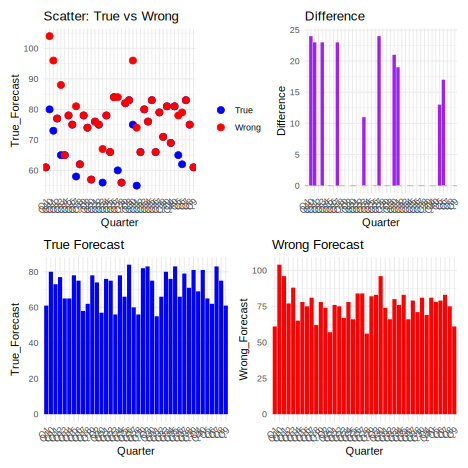
\includegraphics[keepaspectratio]{small-errors-big-consequences-final_files/figure-pdf/unnamed-chunk-6-1.pdf}}

\pandocbounded{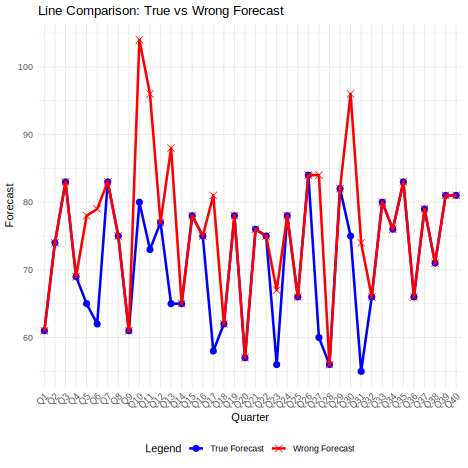
\includegraphics[keepaspectratio]{small-errors-big-consequences-final_files/figure-pdf/unnamed-chunk-7-1.pdf}}

\textbf{Case Study: Forecasting Error in Financial Reports}

A company (we'll simulate Samsung) published quarterly revenue
forecasts. Due to a data entry error, some forecasts were overstated,
misleading stakeholders and resulting in strategic misalignment.

(\citeproc{ref-yahoo_samsung_analysis}{\textbf{yahoo\_samsung\_analysis?}})

Dataset (Simulated) :

Plot --- Comparison Between True vs Wrong Forecast :

\pandocbounded{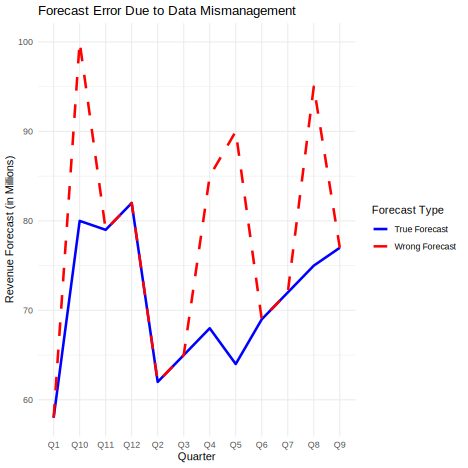
\includegraphics[keepaspectratio]{small-errors-big-consequences-final_files/figure-pdf/unnamed-chunk-9-1.pdf}}

Plot --- Difference Between Forecasts :

\pandocbounded{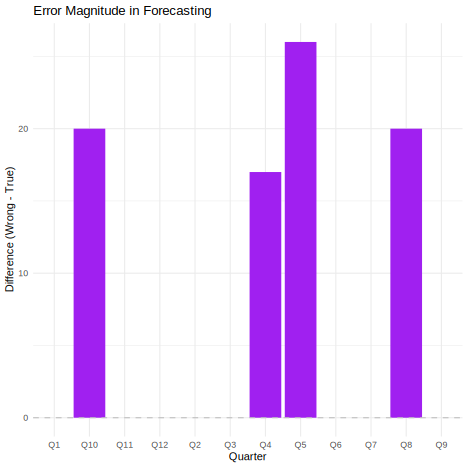
\includegraphics[keepaspectratio]{small-errors-big-consequences-final_files/figure-pdf/unnamed-chunk-10-1.pdf}}

Even small data entry errors in financial forecasts can result in severe
consequences: stakeholder confusion, misplaced budgets, reputational
damage, and market response volatility. Validating data before
publication is not optional---it's critical.

(\citeproc{ref-unknown_nodate_valuableinfo}{Unknown, n.d.})

\textbf{This is a tangible example that I experienced years ago :}

Some times ago I tried to write a program which is related to the
detection and prediction of breast cancer cells.

The program worked in a way that could recognized cancer cells from
healthy cells (malignant cells and benign cells) based on color or
black-and-white imaging (color spectrum) of the breast and was designed
to locate the origin.

The program was connecting to a robot, which would identify the
coordinates of cancer cells using 3D imaging and then begin laser
therapy.

\textbf{Why use a robot?}

To minimize human error. This method is typically effective for
eliminating very small, early-stage tumors (Laser Ablation). The robot
was supposed to irradiate the area around each malignant cell with a
margin of error between 1 to 7 nanometers.

However, the programming encountered some flaws and failed to accurately
identify malignant cells based on color spectrum analysis. As a result,
instead of targeting the cancerous cells, the laser mistakenly hit
surrounding healthy cells, causing unintended burns. This was a small
but clear example of \textbf{``Small Errors, Big Consequences.''}

Some Codes that showing the plot in 2D and 3D :

\textbf{2D Visualization} (PCA on Breast Cancer Dataset) :

\pandocbounded{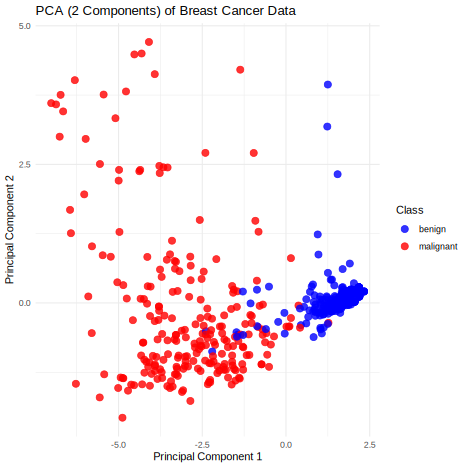
\includegraphics[keepaspectratio]{small-errors-big-consequences-final_files/figure-pdf/unnamed-chunk-11-1.pdf}}

\textbf{3D Visualization (PCA on Breast Cancer Dataset) :}

\pandocbounded{\includegraphics[keepaspectratio]{small-errors-big-consequences-final_files/figure-pdf/unnamed-chunk-12-1.pdf}}

\textbf{The green spot} was the area where we grew the cancer cells.
However, due to an error, this green area, which should have been
exposed to the laser radiation, was not, and it caused damage to other
tissues.

\begin{figure}[H]

\caption{Fig1.Errors Lazering}

{\centering \pandocbounded{\includegraphics[keepaspectratio]{mouse002.jpg}}

}

\end{figure}%

As you can see in the image above, the red area in the fourth photo is
the cancerous tissue, and the green area is the part that was mistakenly
treated with laser therapy.

\section{Conclusion}\label{conclusion}

In an era where data drives every aspect of business operations and
strategic decision-making, the integrity and management of data have
become paramount. This paper has demonstrated that even minor errors in
data---whether originating from manual entry, faulty algorithms,
outdated sources, or insufficient validation---can result in severe,
sometimes irreversible, consequences for organizations. Through detailed
examples and real-world business cases, it has become clear that poor
data quality and mismanagement are not just technical issues but
strategic vulnerabilities that threaten financial stability, operational
efficiency, regulatory compliance, and organizational reputation.

The cost of bad data is not limited to direct financial losses. As seen
in cases ranging from Samsung's market value drop due to a data entry
error, to the Equifax data breach, the ripple effects include loss of
stakeholder trust, missed market opportunities, and long-term
reputational harm. The medical technology example highlighted how data
errors can even impact human lives, underlining the critical importance
of robust data governance and validation at every stage---from
collection and storage to analysis and action.

The lessons are clear: businesses must treat data as a strategic asset.
This means investing in comprehensive data governance frameworks,
adopting best practices in validation and normalization, ensuring
cross-departmental integration, and providing ongoing staff training. By
proactively identifying and mitigating sources of data error,
organizations can transform data from a potential liability into a
foundation for innovation, competitive advantage, and sustainable
success.

Ultimately, the path forward is not simply about avoiding mistakes, but
about building resilient systems and cultures that recognize the value
of data---and the potentially massive consequences of even the smallest
errors.

\section{References}\label{references}

\phantomsection\label{refs}
\begin{CSLReferences}{1}{0}
\bibitem[\citeproctext]{ref-kitchin2014data}
Kitchin, R. (2014). \emph{The data revolution: Big data, open data, data
infrastructures and their consequences}. Sage Publications.

\bibitem[\citeproctext]{ref-provost2013data}
Provost, F., \& Fawcett, T. (2013). \emph{Data science for business:
What you need to know about data mining and data-analytic thinking}.
O'Reilly Media.

\bibitem[\citeproctext]{ref-unknown_nodate_valuableinfo}
Unknown. (n.d.). \emph{Discusses what makes information valuable or
harmful in decision-making processes}.

\end{CSLReferences}

\section{Affidavit}\label{affidavit}

I hereby affirm that this submitted paper was authored unaided and
solely by me. Additionally, no other sources than those in the reference
list were used. Parts of this paper, including tables and figures, that
have been taken either verbatim or analogously from other works have in
each case been properly cited with regard to their origin and
authorship. This paper either in parts or in its entirety, be it in the
same or similar form, has not been submitted to any other examination
board and has not been published.

I acknowledge that the university may use plagiarism detection software
to check my thesis. I agree to cooperate with any investigation of
suspected plagiarism and to provide any additional information or
evidence requested by the university.

Checklist:

\begin{itemize}
\tightlist
\item[$\boxtimes$]
  The handout contains 3-5 pages of text.
\item[$\boxtimes$]
  The submission contains the Quarto file of the handout.
\item[$\boxtimes$]
  The submission contains the Quarto file of the presentation.
\item[$\boxtimes$]
  The submission contains the HTML file of the handout.
\item[$\boxtimes$]
  The submission contains the HTML file of the presentation.
\item[$\boxtimes$]
  The submission contains the PDF file of the handout.
\item[$\boxtimes$]
  The submission contains the PDF file of the presentation.
\item[$\boxtimes$]
  The title page of the presentation and the handout contain personal
  details (name, email, matriculation number).
\item[$\boxtimes$]
  The handout contains a abstract.
\item[$\boxtimes$]
  The presentation and the handout contain a bibliography, created using
  BibTeX with APA citation style.
\item[$\boxtimes$]
  Either the handout or the presentation contains R code that proof the
  expertise in coding.
\item[$\boxtimes$]
  The handout includes an introduction to guide the reader and a
  conclusion summarizing the work and discussing potential further
  investigations and readings, respectively.
\item[$\boxtimes$]
  All significant resources used in the report and R code development.
\item[$\boxtimes$]
  The filled out Affidavit.
\item[$\boxtimes$]
  A concise description of the successful use of Git and GitHub, as
  detailed here: \url{https://github.com/hubchev/make_a_pull_request}.
\item[$\boxtimes$]
  The link to the presentation and the handout published on GitHub.
\end{itemize}

{[}Alireza Toutounchi,{]} {[}06/18/2025,{]} {[}Koln{]}






\end{document}
